\documentclass{beamer}

\mode<presentation> {
\usetheme{Madrid}
\usecolortheme{beaver}
\setbeamertemplate{footline}[page number] % To replace the footer line in all slides with a simple slide count uncomment this line
\setbeamertemplate{navigation symbols}{} % To remove the navigation symbols from the bottom of all slides uncomment this line
}

\usepackage{graphicx}
\title[Sensors Assignment 3]
{Scortec ER-I Manipulator Control using Arduino Due}
\author
{Chittaranjan Srinivas Swaminathan \& Anders Wikstrom}
\institute{Orebro University}
\begin{document}
\frame{\titlepage}
  \begin{frame}
    \frametitle{Outline}
    \begin{enumerate}
      \item Description of the task
      \item Required steps
      \item Reverse Engineering
        \begin{itemize}
          \item Pinout diagram
          \item Encoders and debouncing
        \end{itemize}
      \item Control
        \begin{itemize}
          \item Velocity Control
          \item Position Control
          \item Calibration
        \end{itemize}
      \item Accuracy and precision
        \begin{itemize}
          \item Measurement 
          \item Control
        \end{itemize}
    \end{enumerate}

  \end{frame}
  \begin{frame}
    \frametitle{The task}
    \centering
    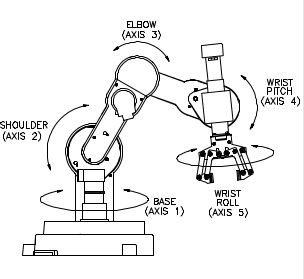
\includegraphics[scale=0.75]{../Report/axes.png}
    \begin{itemize}
      \item<1-> Scortex ER-I, 5-DOF manipulator. Control Box missing.
      \item<2-> Use Arduino Due + Motor shield and make a new controller.
    \end{itemize}
  \end{frame}

  \begin{frame}
    \frametitle{Required Steps}
    \begin{enumerate}
    \item<1-> Reverse engineer the connections and make a pinout
      diagram.
    \item<2-> Program the microcontroller to read the encoders and verify it.
      \begin{itemize}
      \item<2-> We ran into problems here...
      \end{itemize}
    \item<3-> Write control routines for position and velocity control.
    \item<4-> Extend the control routines to more than one joint.
    \item<5-> Measure Accuracy and Precision.
    \end{enumerate}
  \end{frame}
  
  \begin{frame}
    \frametitle{Reverse engineering}
    \begin{enumerate}
      \item<1-> Technique: use the continuity test on the multimeter
        and trace out the wires/pins. 
      \item<2-> For encoders:
        \begin{itemize}
          \item<2-> First relate the pins on D50 connector to the pins
            on the encoder board.
          \item<3-> Then figure out the circuitry so that we know
            what each pin means.
        \end{itemize}
      \item<4-> Connect these pins to the Arduino and read the
        encoders. 
    \end{enumerate}
  \end{frame}

  \begin{frame}
    \frametitle{The pinout diagram for D50 connector}
    \centering
    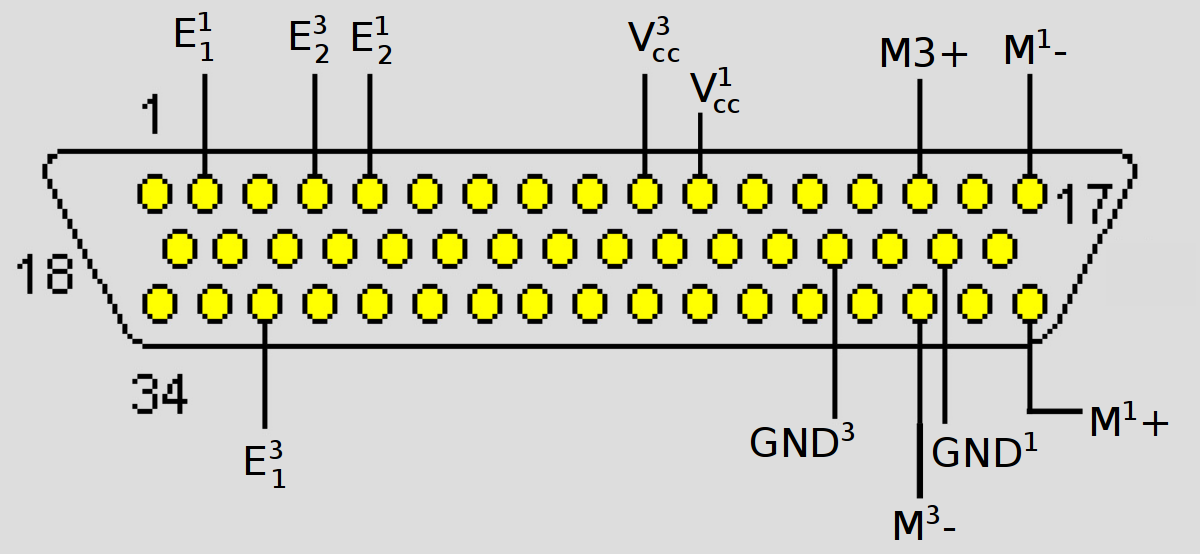
\includegraphics[scale=0.25]{../Report/dsub50.png}
    \begin{itemize}
      \item \( E^a_b \) - output of encoder \textit{b} on joint
        \textit{a}.
      \item \( GND^a \) - ground for encoder board on joint
        \textit{a}.
      \item \( V^a_{cc} \) - power supply for encoder board on joint
        \textit{a}.
      \item \( M^a+ \) - the positive pin on motor \textit{a}.
      \item \( M^a- \) - the negative pin on motor \textit{a}.
      \end{itemize}
  \end{frame}

  \begin{frame}
    \centering
    \frametitle{Encoder circuit}
    \begin{tabular}{p{0.5\textwidth} p{0.45\textwidth}}
      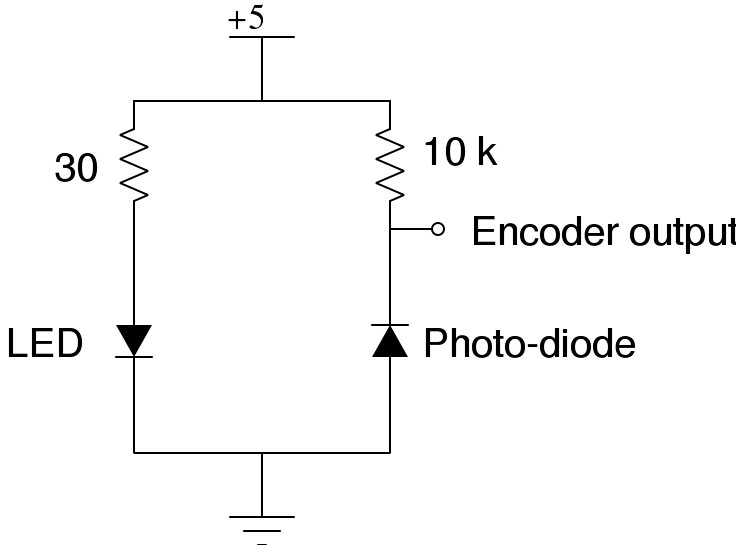
\includegraphics[scale=0.25]{../Report/SimpleEncoder.jpg} &
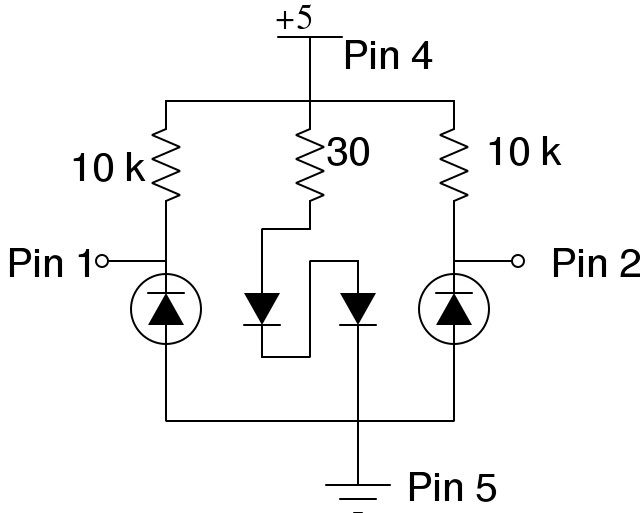
\includegraphics[scale=0.25]{../Report/EncoderCircuit.jpg} \\
      Simple circuit for a Photodiode-LED pair. &
Equivalent circuit for the encoder board.
    \end{tabular}
  \end{frame}

  \begin{frame}
    
    \frametitle{Problems with the encoders}
    Then we did the following:
    \begin{itemize}
    \item<2-> Connect the encoders and write routines\footnote{We took the routines from
    \url{http://playground.arduino.cc/Main/RotaryEncoders}.} to read the
      encoders.
    \item<3-> Move the motor shaft by hand (using the encoder flange) and
      verify the readings.
    \item<4-> Move the joint by hand and note the number of readings.
    \item<5-> Move the joint using PWM and compare it with the one above.
    \end{itemize}
    
    \onslide<6-> The importance of last two steps were discovered by chance.\\
  \end{frame}
  
  \begin{frame}
    \frametitle{Debouncer circuit}
    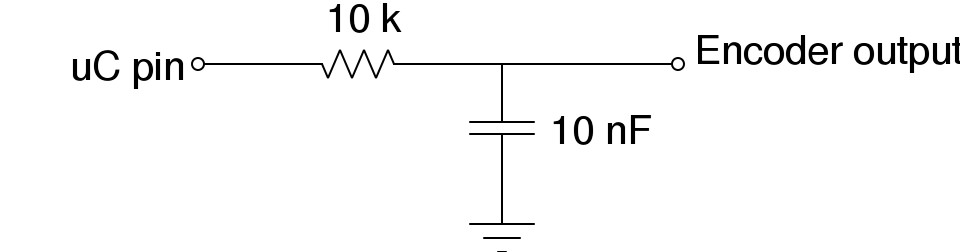
\includegraphics[scale=0.3]{../Report/debouncer.jpg}\\
    \vspace{1cm}
    \begin{itemize}
    \item<1-> A debouncer was required.
    \item<2-> Debouncer is a  simple RC filter.
    \item<3-> The different encoder readings were similar after
    introduction of the debouncer.
    \end{itemize}
  \end{frame}
  
\end{document}